\chapter{Repository, Staging Area e Commit}

\section*{Introduzione}
Questo capitolo copre le operazioni fondamentali di Git: inizializzare repository, gestire la staging area, creare commit significativi, visualizzare la storia e configurare file da ignorare. Questi sono i comandi che userai quotidianamente nel lavoro con Git.

\section*{Obiettivi di apprendimento}
\begin{itemize}
    \item Inizializzare repository Git (\texttt{git init})
    \item Comprendere il ruolo della staging area
    \item Creare commit con messaggi descrittivi
    \item Visualizzare stato e storia del repository
    \item Configurare .gitignore per escludere file
    \item Navigare la storia dei commit con git log
    \item Comprendere le best practices per commit atomici
\end{itemize}

\section{Inizializzare un Repository Git}

\subsection{Creare un nuovo repository}

Per iniziare a tracciare un progetto con Git, devi inizializzare un repository:

\begin{lstlisting}[caption=Inizializzare repository Git]
# Crea directory progetto
$ mkdir mio-progetto
$ cd mio-progetto

# Inizializza repository Git
$ git init
Initialized empty Git repository in /home/user/mio-progetto/.git/

# Verifica creazione directory .git
$ ls -la
drwxr-xr-x  .git/
\end{lstlisting}

\textbf{Cosa succede}:
\begin{itemize}
    \item Git crea directory nascosta \texttt{.git/}
    \item Contiene database, configurazione, refs, hooks
    \item La directory \texttt{.git/} è il repository vero e proprio
    \item La directory di lavoro è ora tracciata da Git
\end{itemize}

\begin{tcolorbox}[colback=orange!10, colframe=orange!60, title=Attenzione: Directory .git]
\textbf{Mai eliminare o modificare manualmente} la directory \texttt{.git/}. Contiene tutta la storia del progetto. Eliminarla significa perdere tutto il version control (i file rimarranno, ma senza storia).
\end{tcolorbox}

\subsection{Struttura directory .git}

\begin{lstlisting}[caption=Contenuto directory .git]
$ tree .git -L 1
.git/
├── HEAD                 # Puntatore al branch corrente
├── config               # Configurazione repository-specific
├── description          # Descrizione repository (GitWeb)
├── hooks/               # Script hook personalizzati
├── index                # Staging area (file binario)
├── info/                # Exclude patterns globali
├── objects/             # Database oggetti Git (blob, tree, commit)
└── refs/                # Puntatori a commit (branches, tags)
\end{lstlisting}

\textbf{File/Directory chiave}:
\begin{description}
    \item[\texttt{HEAD}] Puntatore simbolico al branch corrente (es: \texttt{ref: refs/heads/main})
    \item[\texttt{index}] Staging area (snapshot file pronti per commit)
    \item[\texttt{objects/}] Database content-addressable con tutti gli oggetti
    \item[\texttt{refs/heads/}] Puntatori ai commit di ogni branch
\end{description}

\subsection{Clonare repository esistente}

Alternativa a \texttt{git init}: clonare repository esistente.

\begin{lstlisting}[caption=Clonare repository remoto]
# Clona da GitHub
$ git clone https://github.com/username/repo.git

# Clona con nome directory custom
$ git clone https://github.com/username/repo.git mio-nome

# Clona solo ultimo commit (shallow clone)
$ git clone --depth 1 https://github.com/username/repo.git
\end{lstlisting}

Clone crea:
\begin{itemize}
    \item Copia completa del repository (storia inclusa)
    \item Configurazione automatica remote "origin"
    \item Checkout automatico branch di default
\end{itemize}

\section{La Staging Area (Index)}

\subsection{Concetto di staging area}

La \textbf{staging area} (o index) è una caratteristica distintiva di Git. È un'area intermedia tra working directory e repository.

\begin{figure}[h]
    \centering
    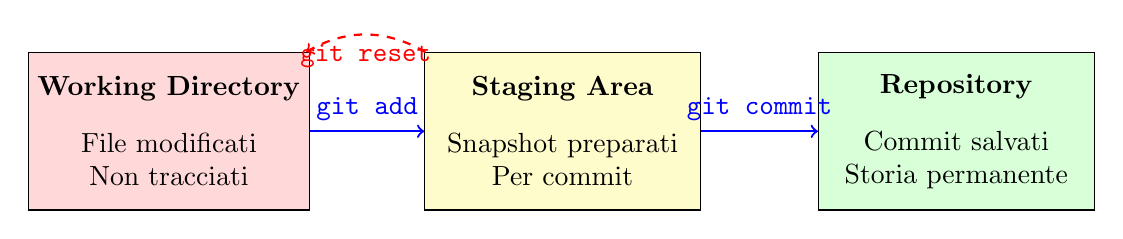
\begin{tikzpicture}[
        box/.style={rectangle, draw, minimum width=3.5cm, minimum height=2cm, align=center},
        arrow/.style={->, thick}
    ]
        % Boxes
        \node[box, fill=red!15] (wd) at (0,0) {
            \textbf{Working Directory}\\[0.3cm]
            File modificati\\
            Non tracciati
        };

        \node[box, fill=yellow!20] (sa) at (5,0) {
            \textbf{Staging Area}\\[0.3cm]
            Snapshot preparati\\
            Per commit
        };

        \node[box, fill=green!15] (repo) at (10,0) {
            \textbf{Repository}\\[0.3cm]
            Commit salvati\\
            Storia permanente
        };

        % Arrows
        \draw[arrow, blue] (wd) -- node[above] {\texttt{git add}} (sa);
        \draw[arrow, blue] (sa) -- node[above] {\texttt{git commit}} (repo);
        \draw[arrow, red, dashed] (sa) to[bend right=30] node[below] {\texttt{git reset}} (wd);
    \end{tikzpicture}
    \caption{Flusso attraverso staging area}
\end{figure}

\textbf{Perché staging area?}
\begin{itemize}
    \item \textbf{Controllo granulare}: Scegli esattamente cosa committare
    \item \textbf{Commit parziali}: Committi solo parte delle modifiche
    \item \textbf{Review pre-commit}: Verifica cosa stai per committare
    \item \textbf{Commit atomici}: Raggruppa modifiche logicamente correlate
\end{itemize}

\begin{tcolorbox}[colback=blue!10, colframe=blue!60, title=Esempio: Staging Parziale]
Hai modificato 5 file:
\begin{itemize}
    \item 3 file implementano feature A
    \item 2 file implementano feature B
\end{itemize}

Con staging area puoi fare:
\begin{enumerate}
    \item \texttt{git add} solo i 3 file di feature A
    \item \texttt{git commit -m "Add feature A"}
    \item \texttt{git add} i 2 file di feature B
    \item \texttt{git commit -m "Add feature B"}
\end{enumerate}

Risultato: Due commit separati e logici, non un commit confuso con entrambe le feature.
\end{tcolorbox}

\subsection{Stati dei file in Git}

File in Git hanno quattro stati possibili:

\begin{description}
    \item[\textbf{Untracked}] File nuovo, Git non lo sta tracciando
    \item[\textbf{Unmodified}] File tracciato, non modificato dall'ultimo commit
    \item[\textbf{Modified}] File tracciato e modificato, non in staging
    \item[\textbf{Staged}] File in staging area, pronto per commit
\end{description}

\begin{figure}[h]
    \centering
    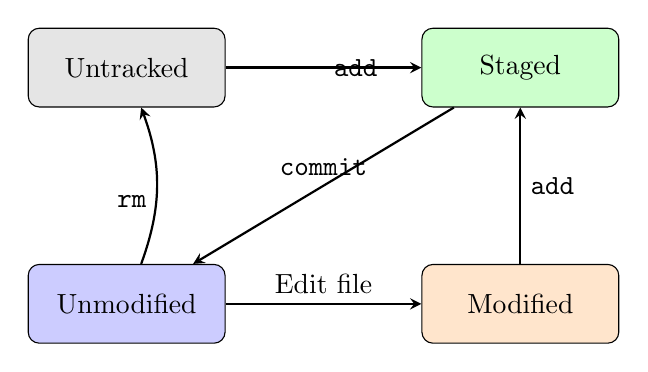
\begin{tikzpicture}[
        state/.style={rectangle, rounded corners, draw, minimum width=2.5cm, minimum height=1cm, align=center},
        arrow/.style={->, >=stealth, thick}
    ]
        \node[state, fill=gray!20] (untracked) at (0,3) {Untracked};
        \node[state, fill=blue!20] (unmodified) at (0,0) {Unmodified};
        \node[state, fill=orange!20] (modified) at (5,0) {Modified};
        \node[state, fill=green!20] (staged) at (5,3) {Staged};

        \draw[arrow] (untracked) -- node[right, pos=0.5] {\texttt{add}} (staged);
        \draw[arrow] (staged) -- node[above] {\texttt{commit}} (unmodified);
        \draw[arrow] (unmodified) -- node[above] {Edit file} (modified);
        \draw[arrow] (modified) -- node[right] {\texttt{add}} (staged);
        \draw[arrow] (unmodified) to[bend right=20] node[below left] {\texttt{rm}} (untracked);
    \end{tikzpicture}
    \caption{Ciclo di vita degli stati dei file}
\end{figure}

\section{Visualizzare lo Stato: git status}

\subsection{Comando git status}

\texttt{git status} è il comando più usato: mostra stato di working directory e staging area.

\begin{lstlisting}[caption=Esempio git status]
$ git status
On branch main

No commits yet

Untracked files:
  (use "git add <file>..." to include in what will be committed)
        README.md
        main.py

nothing added to commit but untracked files present (use "git add" to track)
\end{lstlisting}

\textbf{Output spiega}:
\begin{itemize}
    \item Branch corrente: \texttt{main}
    \item File untracked: \texttt{README.md}, \texttt{main.py}
    \item Suggerimento: usa \texttt{git add} per tracciare
\end{itemize}

\subsection{git status dopo modifiche}

\begin{lstlisting}[caption=Status con file modificati]
$ echo "Hello World" > README.md
$ git add README.md
$ echo "print('Hello')" > main.py

$ git status
On branch main

No commits yet

Changes to be committed:
  (use "git rm --cached <file>..." to unstage)
        new file:   README.md

Untracked files:
  (use "git add <file>..." to include in what will be committed)
        main.py
\end{lstlisting}

\textbf{Sezioni output}:
\begin{itemize}
    \item \textbf{Changes to be committed}: File in staging (README.md)
    \item \textbf{Untracked files}: File non tracciati (main.py)
\end{itemize}

\subsection{Status compatto}

\begin{lstlisting}[caption=git status in formato breve]
$ git status -s
A  README.md    # Staged (Added)
?? main.py      # Untracked

$ git status --short --branch
## main [ahead 2]
A  README.md
M  config.py    # Modified
?? main.py
\end{lstlisting}

\textbf{Codici status}:
\begin{itemize}
    \item \texttt{??} - Untracked
    \item \texttt{A} - Added (staged)
    \item \texttt{M} - Modified
    \item \texttt{D} - Deleted
    \item \texttt{R} - Renamed
    \item \texttt{MM} - Modified sia in staging che in working directory
\end{itemize}

\section{Aggiungere File: git add}

\subsection{Staging di file}

\begin{lstlisting}[caption=git add - aggiungere file]
# Aggiungi file singolo
$ git add README.md

# Aggiungi più file
$ git add main.py utils.py config.py

# Aggiungi tutti i file con estensione
$ git add *.py

# Aggiungi tutti i file nella directory
$ git add src/

# Aggiungi tutti i file modificati e nuovi
$ git add .

# Aggiungi tutti (inclusi file eliminati)
$ git add -A
# Equivalente a:
$ git add --all
\end{lstlisting}

\subsection{Staging interattivo}

\begin{lstlisting}[caption=git add interattivo]
# Modalità interattiva (permette scelta selettiva)
$ git add -i

# Staging patch-by-patch (scegli singoli chunk)
$ git add -p

# Esempio output git add -p:
diff --git a/main.py b/main.py
@@ -1,3 +1,4 @@
 def hello():
     print("Hello")
+    print("World")

Stage this hunk [y,n,q,a,d,s,e,?]?
# y = yes, n = no, s = split, e = edit, ? = help
\end{lstlisting}

\begin{tcolorbox}[colback=green!10, colframe=green!60, title=Best Practice: git add -p]
\texttt{git add -p} è estremamente utile quando hai fatto molte modifiche ma vuoi committare solo parte di esse. Ti permette di creare commit atomici anche quando hai lavorato su più cose contemporaneamente.
\end{tcolorbox}

\subsection{Unstaging: rimuovere da staging}

\begin{lstlisting}[caption=Rimuovere file da staging area]
# Rimuovi file da staging (Git 2.23+)
$ git restore --staged README.md

# Metodo old-school (funziona sempre)
$ git reset HEAD README.md

# Rimuovi tutti i file da staging
$ git reset HEAD .
\end{lstlisting}

\section{Creare Commit: git commit}

\subsection{Commit base}

Un \textbf{commit} è uno snapshot permanente dei file in staging area.

\begin{lstlisting}[caption=Creare commit]
# Commit con messaggio inline
$ git commit -m "Add README with project description"
[main (root-commit) a3f5b21] Add README with project description
 1 file changed, 3 insertions(+)
 create mode 100644 README.md

# Commit apre editor per messaggio multi-line
$ git commit
# Editor si apre, scrivi messaggio, salva e chiudi
\end{lstlisting}

\textbf{Output commit spiega}:
\begin{itemize}
    \item Branch: \texttt{main}
    \item Hash commit: \texttt{a3f5b21} (abbreviato da 40 caratteri)
    \item File cambiati: 1
    \item Inserimenti: 3 righe
\end{itemize}

\subsection{Commit con add automatico}

\begin{lstlisting}[caption=Commit skip staging (solo file tracciati)]
# Aggiungi e committi in un comando (solo modified files)
$ git commit -a -m "Update all tracked files"

# Equivalente a:
$ git add -u   # Aggiungi solo file già tracciati modificati
$ git commit -m "Update all tracked files"
\end{lstlisting}

\begin{tcolorbox}[colback=red!10, colframe=red!60, title=Attenzione: git commit -a]
\texttt{git commit -a} aggiunge automaticamente solo file \textbf{già tracciati}. File nuovi (untracked) sono ignorati. È comodo ma può causare commit accidentali. Meglio usare \texttt{git add} esplicitamente.
\end{tcolorbox}

\subsection{Anatomia di un buon commit message}

\begin{lstlisting}[caption=Formato commit message]
# Formato standard:
Short summary (50 chars max)

Detailed explanation if needed. Wrap at 72 characters.
Explain WHAT changed and WHY, not HOW (code shows how).

- Bullet points are ok
- Use imperative mood: "Add feature" not "Added feature"

Fixes #123
\end{lstlisting}

\textbf{Best practices commit message}:
\begin{enumerate}
    \item \textbf{Prima riga}: Summary breve (50 caratteri max)
    \item \textbf{Riga vuota}: Separa summary da body
    \item \textbf{Body}: Spiegazione dettagliata (72 caratteri per riga)
    \item \textbf{Imperative mood}: "Add", "Fix", "Update" (non "Added", "Fixed")
    \item \textbf{Perché, non come}: Spiega motivazione, non implementazione
    \item \textbf{References}: Link issue/ticket se presenti
\end{enumerate}

\begin{tcolorbox}[colback=blue!10, colframe=blue!60, title=Esempio Commit Message]
\textbf{Bad}:
\begin{verbatim}
Fixed bug
\end{verbatim}

\textbf{Good}:
\begin{verbatim}
Fix null pointer exception in user login

The login function didn't check if username was null
before accessing length property. This caused crashes
when users submitted empty form.

Now we validate input before processing.

Fixes #456
\end{verbatim}
\end{tcolorbox}

\subsection{Commit atomici}

\textbf{Commit atomico}: Contiene modifiche logicamente correlate a un singolo scopo.

\textbf{Vantaggi}:
\begin{itemize}
    \item Storia leggibile e comprensibile
    \item Facile fare revert di singole feature
    \item Code review più semplice
    \item Bisect più efficace per trovare bug
\end{itemize}

\begin{tcolorbox}[colback=green!10, colframe=green!60, title=Best Practice: Commit Atomici]
\textbf{Do}:
\begin{itemize}
    \item Un commit = una feature/fix
    \item Commit compila e passa test
    \item Message descrive il commit completamente
\end{itemize}

\textbf{Don't}:
\begin{itemize}
    \item Commit con "Fix A and B and refactor C"
    \item Commit che rompe la build
    \item Message generici tipo "Updates" o "WIP"
\end{itemize}
\end{tcolorbox}

\subsection{Ammendare commit}

\begin{lstlisting}[caption=Modificare ultimo commit]
# Hai fatto commit ma dimenticato un file
$ git add forgotten_file.py
$ git commit --amend

# Amend senza cambiare messaggio
$ git commit --amend --no-edit

# Amend cambiando solo messaggio
$ git commit --amend -m "Better commit message"
\end{lstlisting}

\textbf{Cosa fa \texttt{--amend}}:
\begin{itemize}
    \item Sostituisce l'ultimo commit con nuovo commit
    \item Combina staging corrente con commit precedente
    \item Cambia hash commit (tecnicamente nuovo commit)
\end{itemize}

\begin{tcolorbox}[colback=red!10, colframe=red!60, title=Attenzione: Amend dopo Push]
\textbf{Mai fare amend di commit già pushati} su branch condivisi! Amend riscrive la storia. Se altri hanno già pullato quel commit, creerai conflitti. Regola: amend solo commit locali non pushati.
\end{tcolorbox}

\section{Visualizzare Storia: git log}

\subsection{Log base}

\begin{lstlisting}[caption=git log - storia commit]
$ git log
commit a3f5b21e8c9d34f7a2b19c5e6d8f1a4b3c7e9f2d
Author: Mario Rossi <mario@example.com>
Date:   Mon Nov 11 10:30:45 2024 +0100

    Add user authentication feature

commit b8c9d34f7a2b19c5e6d8f1a4b3c7e9f2d3e5a1c
Author: Mario Rossi <mario@example.com>
Date:   Mon Nov 11 09:15:22 2024 +0100

    Initial commit
\end{lstlisting}

\subsection{Log formattato}

\begin{lstlisting}[caption=Formati git log utili]
# Log compatto (una riga per commit)
$ git log --oneline
a3f5b21 Add user authentication feature
b8c9d34 Initial commit

# Log con grafo branch
$ git log --oneline --graph --all
* a3f5b21 (HEAD -> main) Add user authentication
* b8c9d34 Initial commit

# Log dettagliato con file modificati
$ git log --stat
commit a3f5b21...
    auth.py    | 45 ++++++++++++++++++
    login.html | 23 +++++++++
    2 files changed, 68 insertions(+)

# Log con diff completo
$ git log -p
commit a3f5b21...
diff --git a/auth.py b/auth.py
+def login(username, password):
+    # Implementation

# Ultimi N commit
$ git log -n 5      # Ultimi 5 commit
$ git log -3        # Ultimi 3 commit
\end{lstlisting}

\subsection{Filtrare log}

\begin{lstlisting}[caption=Filtrare storia commit]
# Commit di autore specifico
$ git log --author="Mario"

# Commit in range di date
$ git log --since="2024-11-01"
$ git log --since="2 weeks ago"
$ git log --until="2024-11-30"

# Commit che toccano file specifico
$ git log -- README.md
$ git log --follow -- README.md  # Segui rename

# Commit con messaggio contenente keyword
$ git log --grep="bug"
$ git log --grep="feature" --grep="fix"  # OR
$ git log --grep="feature" --all-match   # AND

# Commit che modificano codice specifico
$ git log -S "function_name"  # Pickaxe: cerca nei diff
\end{lstlisting}

\subsection{Log personalizzato}

\begin{lstlisting}[caption=Custom format git log]
# Pretty format personalizzato
$ git log --pretty=format:"%h - %an, %ar : %s"
a3f5b21 - Mario Rossi, 2 hours ago : Add user auth
b8c9d34 - Mario Rossi, 1 day ago : Initial commit

# Formato custom avanzato
$ git log --pretty=format:"%C(yellow)%h%Creset %C(blue)%an%Creset: %s"

# Salva come alias
$ git config --global alias.lg "log --graph --pretty=format:'%Cred%h%Creset -%C(yellow)%d%Creset %s %Cgreen(%cr) %C(bold blue)<%an>%Creset' --abbrev-commit"

$ git lg
* a3f5b21 - (HEAD -> main) Add user auth (2 hours ago) <Mario Rossi>
* b8c9d34 - Initial commit (1 day ago) <Mario Rossi>
\end{lstlisting}

\textbf{Format placeholders utili}:
\begin{itemize}
    \item \texttt{\%h} - Hash abbreviato
    \item \texttt{\%H} - Hash completo
    \item \texttt{\%an} - Author name
    \item \texttt{\%ae} - Author email
    \item \texttt{\%ad} - Author date
    \item \texttt{\%ar} - Author date, relative (2 hours ago)
    \item \texttt{\%s} - Subject (prima riga messaggio)
    \item \texttt{\%b} - Body (resto messaggio)
    \item \texttt{\%d} - Ref names (branch, tag)
\end{itemize}

\section{File .gitignore}

\subsection{Perché .gitignore}

Alcuni file non devono essere tracciati da Git:
\begin{itemize}
    \item File temporanei (\texttt{*.tmp}, \texttt{*.swp})
    \item Build artifacts (\texttt{*.o}, \texttt{*.pyc}, \texttt{dist/})
    \item Dipendenze (\texttt{node\_modules/}, \texttt{venv/})
    \item File IDE (\texttt{.vscode/}, \texttt{.idea/})
    \item Credenziali (\texttt{.env}, \texttt{secrets.json})
    \item File sistema operativo (\texttt{.DS\_Store}, \texttt{Thumbs.db})
\end{itemize}

\subsection{Sintassi .gitignore}

\begin{lstlisting}[caption=Esempio .gitignore]
# Commento

# File specifico
secrets.json

# Pattern wildcard
*.log
*.tmp

# Intere directory
node_modules/
build/
dist/

# Negazione (! = NON ignorare)
*.log
!important.log    # Traccia questo .log specifico

# Ignorare file solo in root
/TODO            # Solo /TODO, non src/TODO

# Ignorare file in qualsiasi subdirectory
**/temp          # Ignora temp ovunque

# Pattern avanzati
**/*.pyc         # .pyc in qualsiasi directory
**/dist/*        # Contenuto di qualsiasi dist/
\end{lstlisting}

\subsection{.gitignore per linguaggi comuni}

\begin{lstlisting}[caption=.gitignore Python]
# Python
__pycache__/
*.py[cod]
*$py.class
*.so
.Python
venv/
env/
ENV/
.pytest_cache/
*.egg-info/
dist/
build/
\end{lstlisting}

\begin{lstlisting}[caption=.gitignore Node.js]
# Node.js
node_modules/
npm-debug.log
yarn-error.log
.env
dist/
build/
.cache/
*.tgz
\end{lstlisting}

\begin{lstlisting}[caption=.gitignore Java]
# Java
*.class
*.jar
*.war
*.ear
target/
.mvn/
.gradle/
build/
\end{lstlisting}

\subsection{Gitignore globale}

\begin{lstlisting}[caption=Configurare gitignore globale]
# Crea file gitignore globale
$ touch ~/.gitignore_global

# Configura Git per usarlo
$ git config --global core.excludesfile ~/.gitignore_global

# Aggiungi pattern OS/IDE comuni
# ~/.gitignore_global
.DS_Store        # macOS
Thumbs.db        # Windows
.vscode/         # VS Code
.idea/           # IntelliJ
*.swp            # Vim
*~               # Backup files
\end{lstlisting}

\subsection{Ignorare file già tracciati}

\begin{lstlisting}[caption=Rimuovere file tracciato da Git]
# Se hai committato file per errore (es: .env)
$ echo ".env" >> .gitignore

# Rimuovi da Git ma mantieni file locale
$ git rm --cached .env

$ git commit -m "Remove .env from tracking"
\end{lstlisting}

\begin{tcolorbox}[colback=red!10, colframe=red!60, title=Errore Comune: .gitignore non funziona]
Se aggiungi pattern a .gitignore ma il file è già tracciato, Git continuerà a tracciarlo. Devi prima fare \texttt{git rm --cached file} per rimuoverlo dall'index.
\end{tcolorbox}

\section{Visualizzare Differenze: git diff}

\subsection{Diff working directory}

\begin{lstlisting}[caption=git diff - vedere modifiche]
# Differenze non staged (working vs staging)
$ git diff
diff --git a/main.py b/main.py
index a3f5b21..b8c9d34 100644
--- a/main.py
+++ b/main.py
@@ -1,3 +1,4 @@
 def hello():
     print("Hello")
+    print("World")

# Differenze staged (staging vs ultimo commit)
$ git diff --staged
$ git diff --cached  # Equivalente

# Differenze completo (working vs ultimo commit)
$ git diff HEAD
\end{lstlisting}

\subsection{Diff tra commit}

\begin{lstlisting}[caption=Diff tra commit specifici]
# Diff tra due commit
$ git diff a3f5b21 b8c9d34

# Diff ultimo commit vs precedente
$ git diff HEAD HEAD~1

# Diff su file specifico
$ git diff main.py
$ git diff a3f5b21 b8c9d34 -- main.py
\end{lstlisting}

\section*{Riepilogo concetti chiave}

\begin{tcolorbox}[colback=gray!10, colframe=black!60, title=Concetti fondamentali]
\begin{itemize}
    \item \texttt{git init} inizializza repository nella directory corrente
    \item \textbf{Staging area} permette controllo granulare su cosa committare
    \item \texttt{git status} mostra stato working directory e staging
    \item \texttt{git add} aggiunge file alla staging area
    \item \texttt{git commit} crea snapshot permanente dei file in staging
    \item \textbf{Commit atomici}: Un commit = una modifica logica
    \item \textbf{Commit message}: Summary breve + body dettagliato
    \item \texttt{git log} visualizza storia commit
    \item \texttt{.gitignore} specifica file da non tracciare
    \item \texttt{git diff} mostra differenze tra versioni
\end{itemize}
\end{tcolorbox}

\section*{Esercizi}

\begin{enumerate}
    \item Crea nuovo repository, aggiungi 3 file e fai primo commit.

    \item Modifica 2 file, usa \texttt{git add -p} per fare commit separati.

    \item Scrivi .gitignore per progetto Python che ignora \texttt{venv/}, \texttt{*.pyc}, \texttt{.env}.

    \item Usa \texttt{git log --oneline --graph} per visualizzare storia.

    \item Fai commit con messaggio multi-line usando editor.

    \item Usa \texttt{git commit --amend} per correggere commit message.

    \item Configura alias \texttt{git lg} per log grafico colorato.

    \item Crea file .gitignore\_global per OS/IDE.

    \item Usa \texttt{git diff} per vedere modifiche prima di committare.

    \item Fai commit di file per errore, usa \texttt{git rm --cached} per rimuoverlo.
\end{enumerate}

\section*{Riferimenti}

\begin{itemize}
    \item Git Basics: \url{https://git-scm.com/book/en/v2/Git-Basics-Getting-a-Git-Repository}
    \item Gitignore templates: \url{https://github.com/github/gitignore}
    \item Commit message guide: \url{https://chris.beams.io/posts/git-commit/}
\end{itemize}
